\section{Марериалы работы}
Рассчитаем коэффициент датчика момента:
\begin{gather*}
    K_M = \frac{U_\text{зад}}{М_\text{зад}}= \frac{U_\text{зад}}{М_\text{ном}}= 0.7299
\end{gather*}

Передаточная функция объекта управления:
\begin{gather*}
    W = \frac{K_M K_\text{пр}\beta}{(T_\text{э}s+1)(T_\text{пр}s+1)}
\end{gather*}

Передаточная функция системы, выполняющей условие технического оптимума:
\begin{gather*}
    W_{MO} = \frac{1}{2T_\mu s(T_\mu s+1)}
\end{gather*}

Передаточная функция ПИ регулятора и ее параметры:
\begin{gather*}
    W_{\text{ПИ}} = \frac{K_p(T_\text{и} s+1)}{T_\text{и} s}\\
    T_{\mu} = T_\text{пр} \\
    T_{и} = T_\text{e}\\
    K_p = \frac{T_e}{2T_\text{пр}K_\text{пр}K_\text{M}\beta}
\end{gather*}
\newpage
Соберем схему моделирования MATLAB Simulink
\begin{figure}[!h]
    \centering
    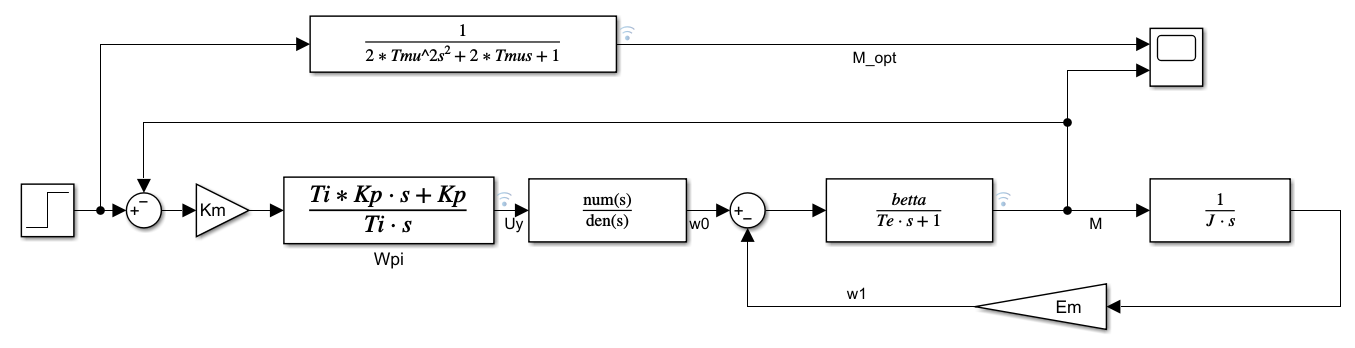
\includegraphics[width=0.9\textwidth]{img/img}
    \caption{Схема моделирования системы}
    \label{fig:matlab}
\end{figure}

Проведем моделирование системы без учета электромеханических связей
\begin{figure}[!h]
    \centering
    \begin{minipage}{0.5\textwidth}
        \centering
        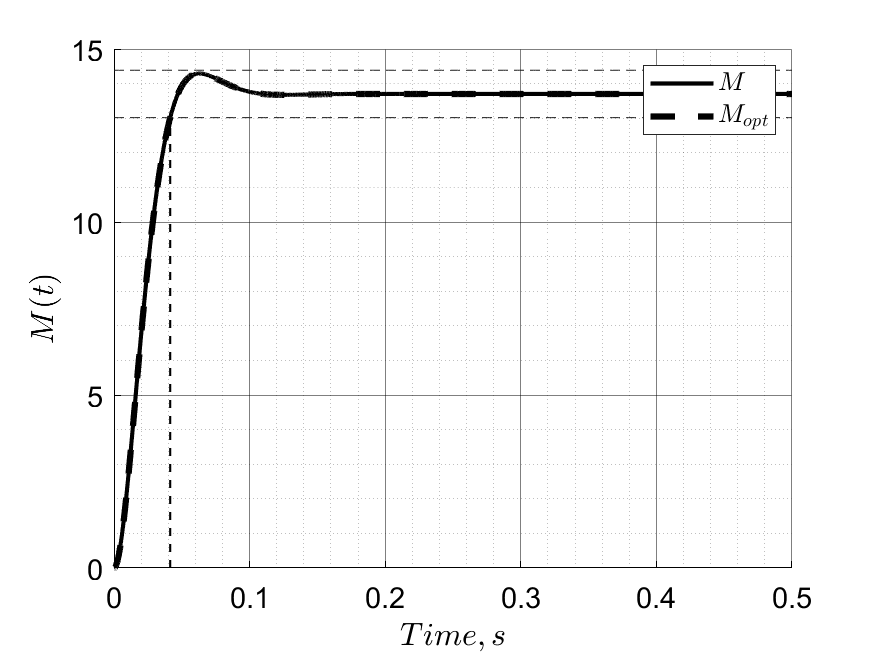
\includegraphics[width = \textwidth]{img/task1_M}
        \caption{График $M(t)$ без электромеханической связи}
        \label{fig:img/task1_M}
    \end{minipage}%
\begin{minipage}{0.5\textwidth}
        \centering
        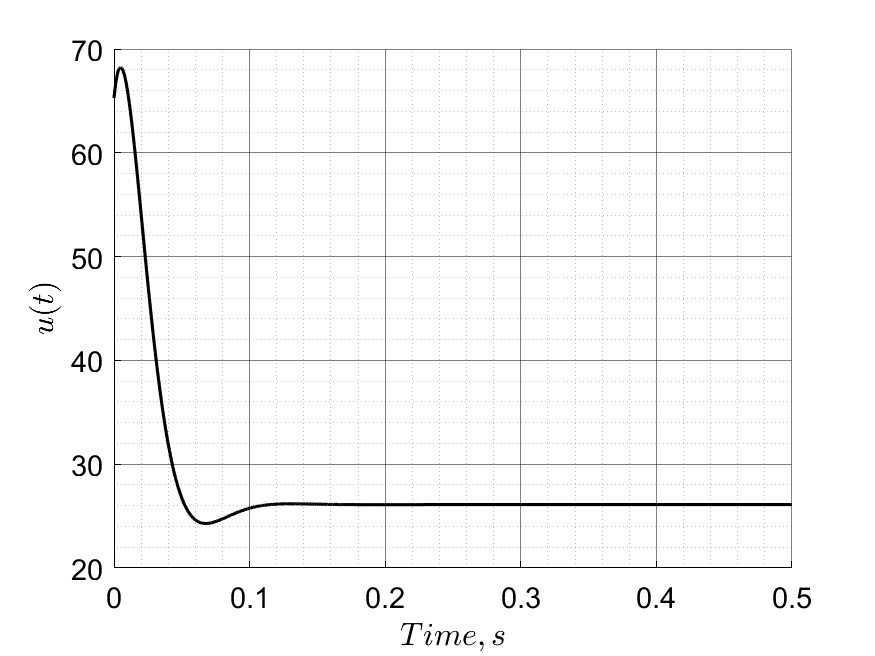
\includegraphics[width = \textwidth]{img/task1_u}
        \caption{График $u(t)$ без электромеханической связи}
        \label{fig:img/task1_u}
    \end{minipage}%
\end{figure}
\begin{figure}[!h]
    \centering
    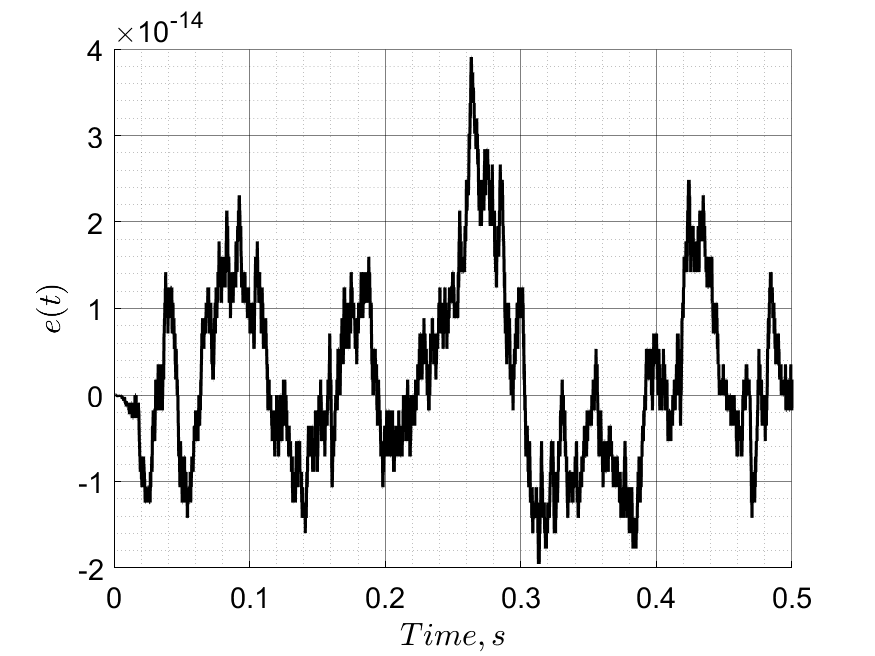
\includegraphics[width=0.5\textwidth]{img/task1_e}
    \caption{График $\varepsilon(t)$ без электромеханической связи}
    \label{fig:task1_e}
\end{figure}

Время переходного процесса: 0.041434 с

Перерегулирование: 4.3214\%
\newpage
Проведем моделирование системы с учетом электромеханических связей
\begin{figure}[!h]
    \centering
    \begin{minipage}{0.5\textwidth}
        \centering
        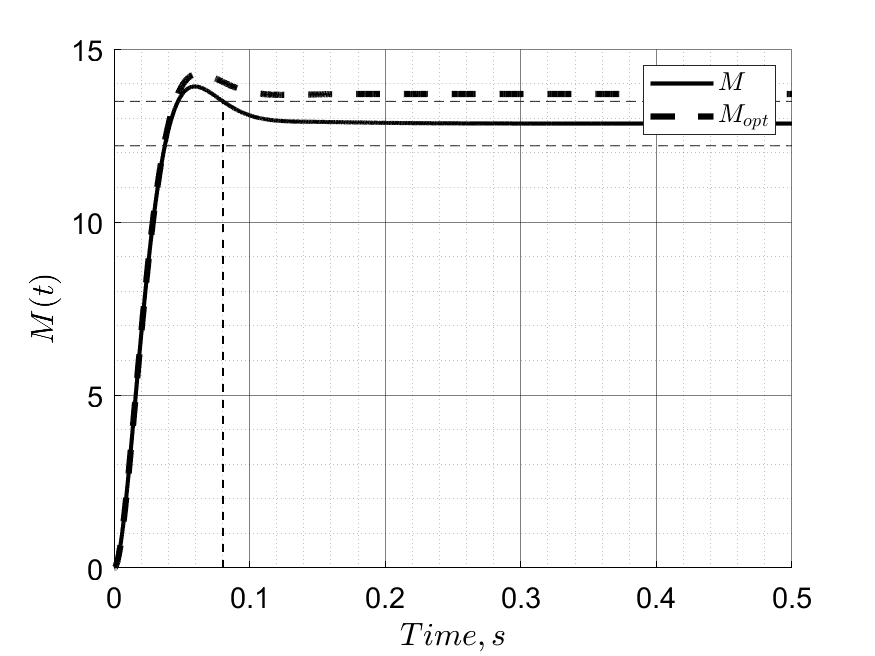
\includegraphics[width = \textwidth]{img/task2_M}
        \caption{График $M(t)$ с учетом электромеханической связи}
        \label{fig:img/task2_M}
    \end{minipage}%
    \begin{minipage}{0.5\textwidth}
        \centering
        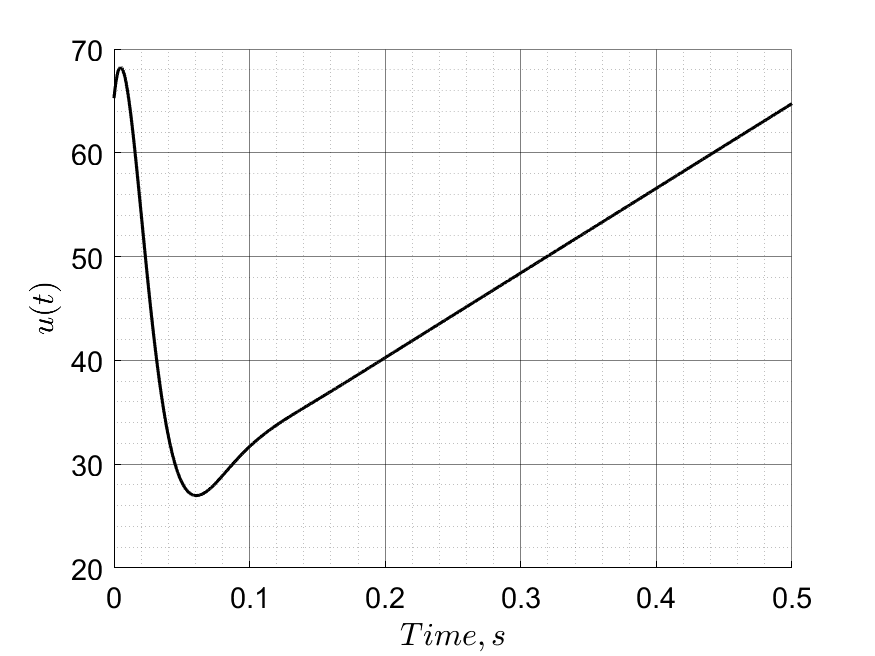
\includegraphics[width = \textwidth]{img/task2_u}
        \caption{График $u(t)$ с учетом электромеханической связи}
        \label{fig:img/task2_u}
    \end{minipage}%
\end{figure}
\begin{figure}[!h]
    \centering
    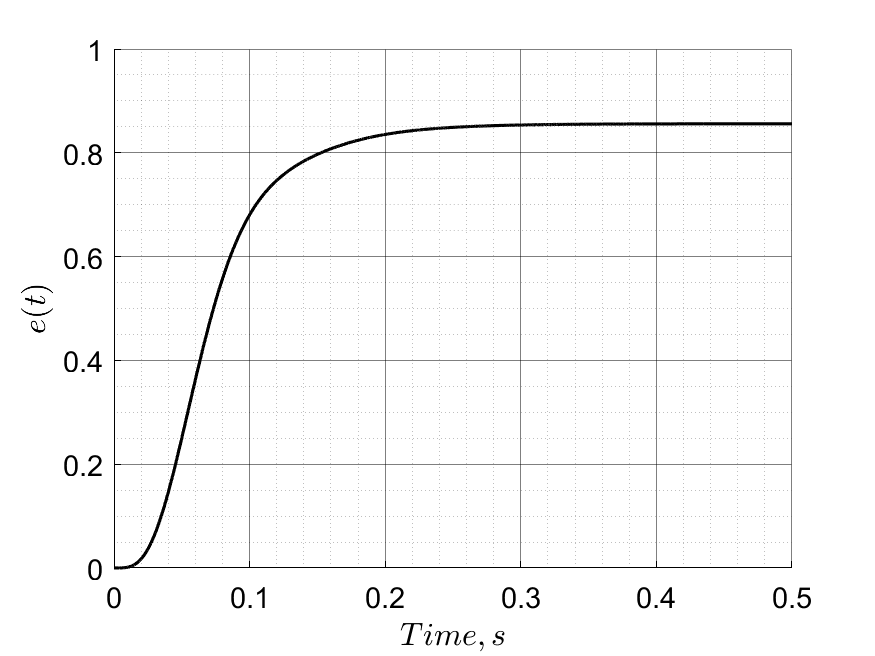
\includegraphics[width=0.5\textwidth]{img/task2_e}
    \caption{График $\varepsilon(t)$ с учетом электромеханической связи}
    \label{fig:task2_e}
\end{figure}

Время переходного процесса: 0.080375 с

Перерегулирование: 8.3481\%